\documentclass[10pt]{beamer}

\usepackage{appendixnumberbeamer}
\usepackage{booktabs}
\usepackage[scale=2]{ccicons}
\usepackage{pgfplots}
\usepackage{graphics}
\usepackage{braket}

\usepgfplotslibrary{dateplot}
\pdfstringdefDisableCommands{\def\translate#1{#1}}
\geometry{paperwidth=140mm, paperheight=105mm}
\usetheme{metropolis}
\bibliographystyle{abbrv}
\setbeamertemplate{frame footer}{ME738 - Special Topics in Materials}

\renewcommand{\footnotesize}{\fontsize{7pt}{8pt}\selectfont}

\title{Chip Scale Atomic Clocks Sources}
\subtitle{Motivations}
\date{March 13, 2024}
\author{Tommaso Bocchietti}
\institute{University of Waterloo}
\titlegraphic{\hfill
\includegraphics[height=1.5cm]{pdf/UniversityOfWaterloo_logo_horiz_pms.pdf}}

\begin{document}

\maketitle

\begin{frame}[fragile]{R\&D direction}

    Program initiated in the early 2000s, funded by DARPA in collaboration with NIST, having the goal of developing an \textbf{ultra-miniaturized, low-power, atomic time and frequency reference units}.

    \begin{figure}[H]
        \centering
        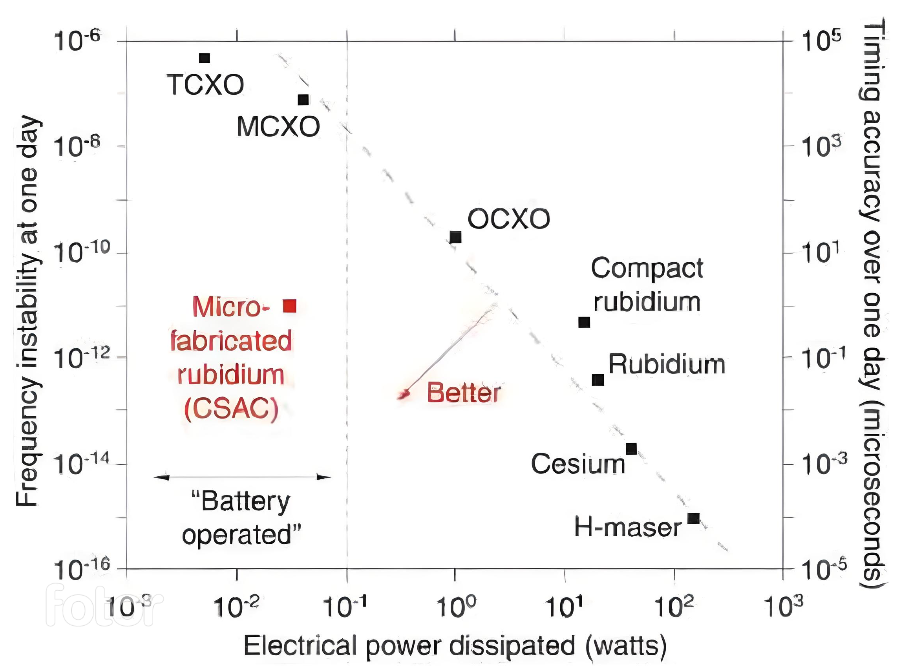
\includegraphics[width=0.6\textwidth]{img/clocks-comparison.png}
    \end{figure}

    Temperature sensitivity, long-term frequency aging, and turn-on to turn-on are better than traditional MEMS based clocks (but still are limiting factors).

\end{frame}



\begin{frame}{Applications}

    Most important applications are related to \textbf{GNSS} (Global Navigation Satellite System).

    Atomically precise timebases for portable, battery-operated GPS receivers allow for improved resistance to jamming and interference, faster acquisition time, and more reliable receiver operation.

    Other applications include:

    \begin{itemize}
        \item Defense applications (i.e. UAVs)
        \item Telecommunications (i.e. next generation 5G networks)
        \item Space experiments (i.e. SPHERES project)
        \item Underwater oil and mineral exploration (through reflection seismology)
    \end{itemize}

\end{frame}



\begin{frame}{Outline for the project}

    Aim for this project is to give an overview of the commercially available CSACs.

    The project will be divided into the following sections:

    \begin{itemize}
        \item \textbf{Working principles}: what's the physics behind the CSACs\footnote{In order to better understand the innovation behind the CSACs, we will also give an overview of the table-size atomic clocks.}
        \item \textbf{Technology comparison}: what are the performances of the different CSACs\footnote{We will also compare the CSACs with the traditional MEMS based clocks and table-size atomic clocks.}
        \item \textbf{Applications}: what's the role of the CSACs in the different applications
        \item \textbf{Future developments}: what are the future perspectives for the CSACs
    \end{itemize}

    Our main focus will be on the Physics Packages (core), disregarding both the Local Oscillator and the Control Electronics.

\end{frame}


\appendix

\begin{frame}[standout]
    Extra slides
\end{frame}



\begin{frame}{Atomic clocks comparison}

    \begin{columns}[c, onlytextwidth]

        \begin{column}{0.25\textwidth}

            \begin{figure}[H]
                \centering
                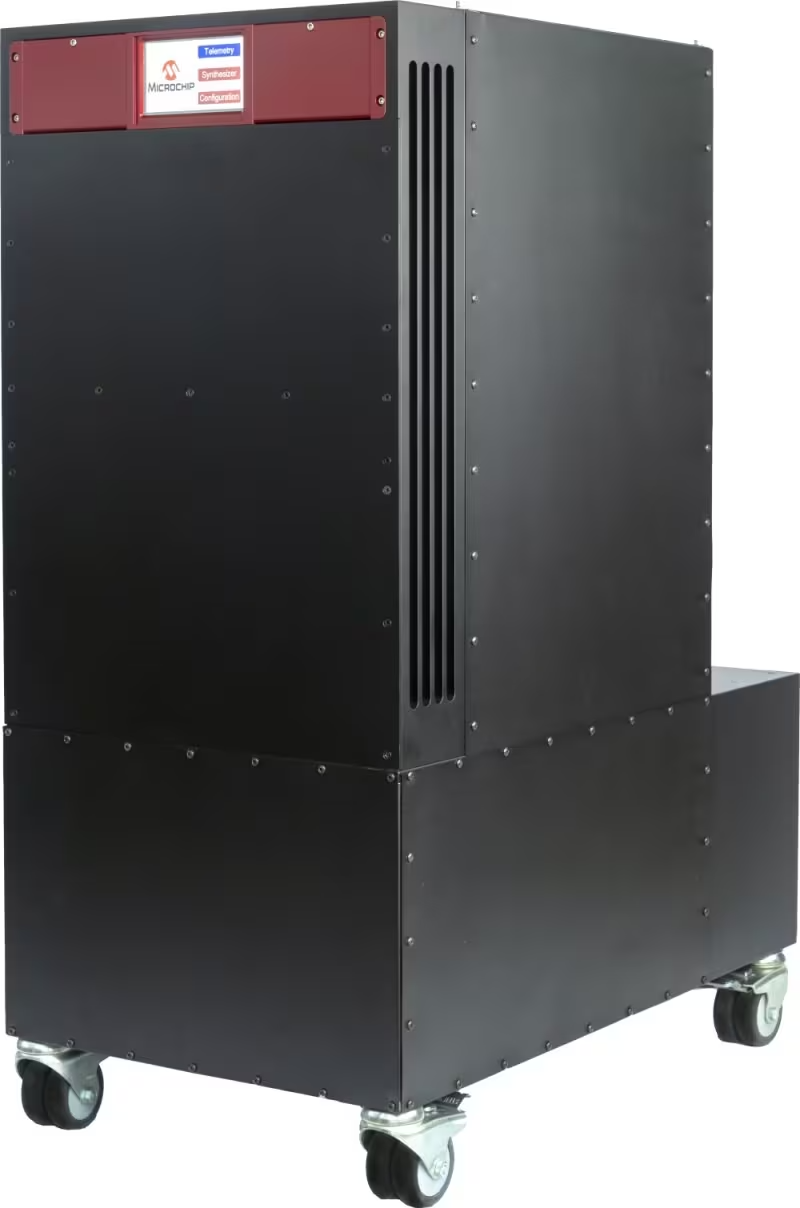
\includegraphics[width=0.9\textwidth]{img/Microsemi-MHM-2020.png}
                \caption{Microsemi MHM 2020}
            \end{figure}

        \end{column}

        \begin{column}{0.25\textwidth}

            \begin{figure}[H]
                \centering
                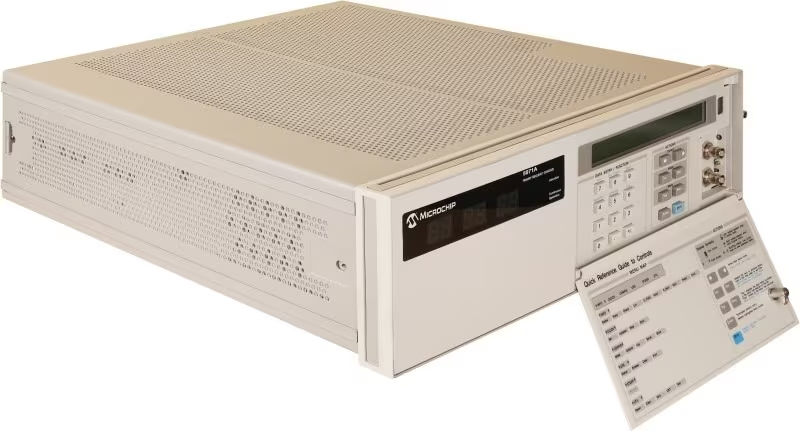
\includegraphics[width=0.9\textwidth]{img/Microsemi-5071A.png}
                \caption{Microsemi 5071A}
            \end{figure}

        \end{column}

        \begin{column}{0.25\textwidth}

            \begin{figure}[H]
                \centering
                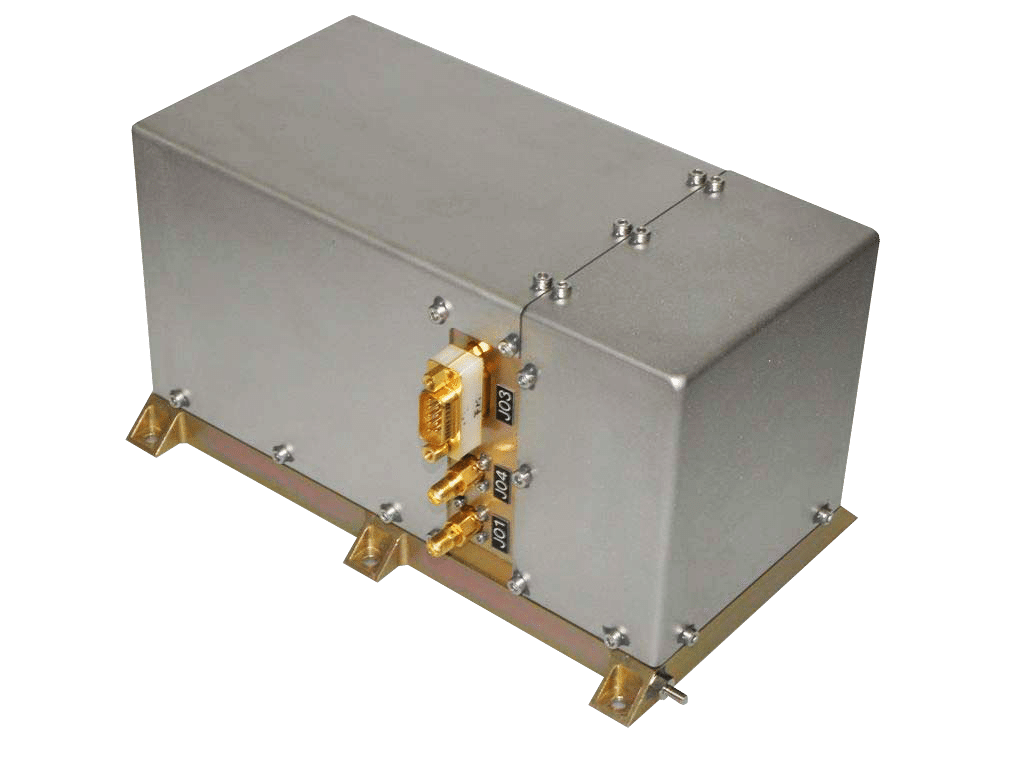
\includegraphics[width=0.9\textwidth]{img/Spectratime-iSpace-RAFS.png}
                \caption{Spectratime iSpace RAFS}
            \end{figure}

        \end{column}

        \begin{column}{0.25\textwidth}

            \begin{figure}[H]
                \centering
                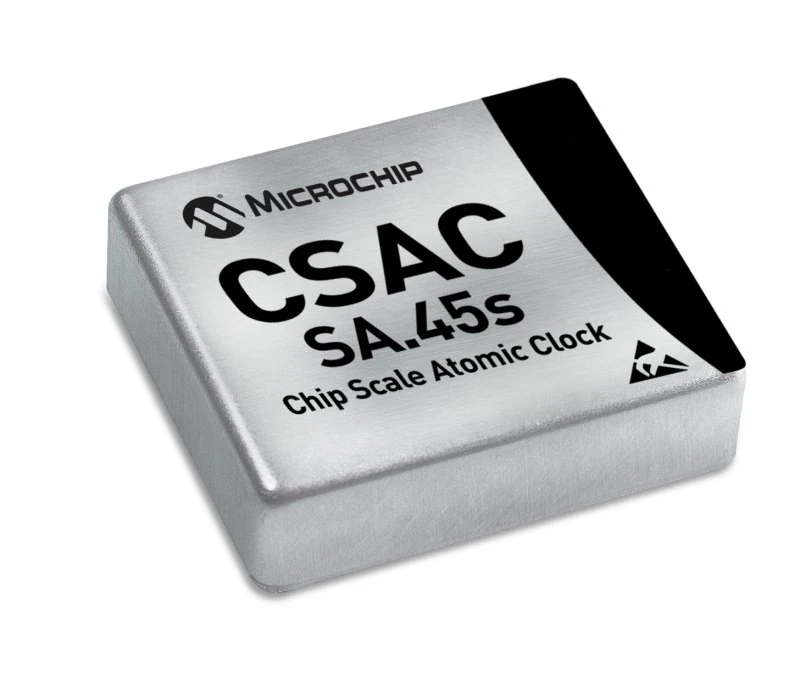
\includegraphics[width=0.9\textwidth]{img/Microsemi-SA45s.png}
                \caption{Microsemi SA45s}
            \end{figure}

        \end{column}

    \end{columns}

    \begin{table}
        \centering

        \resizebox{\columnwidth}{!}{%
            \begin{tabular}{ll|lllllllllll}
                \hline
                \textbf{Vendor} & \textbf{Product} & \textbf{Type} & \textbf{ADEV} & \textbf{Aging} & \textbf{Tmin} & \textbf{Tmax} & \textbf{Tempco} & \textbf{Power} & \textbf{Weight} & \textbf{Size}           \\
                ~               & ~                & ~             & (1 s)         & (month)        & (°C)          & (°C)          & ~               & (W)            & (kg)            & (cm\textsuperscript{3}) \\
                \hline
                Microsemi       & MHM 2020         & Maser         & 8,00E-14      & 9,00E-15       & ~             & ~             & ~               & 75,00          & 246,000         & 374072                  \\
                Microsemi       & 5071A            & CBT           & 5,00E-12      & ~              & 0             & 55            & ~               & 50,00          & 30,000          & 29700                   \\
                Spectratime     & iSpace RAFS      & Space Rb      & 3,00E-12      & 8,30E-12       & -5            & 10            & ~               & 35,00          & 3,400           & 3224                    \\
                Microsemi       & SA45.s           & CSAC          & 3,00E-10      & 9,00E-10       & -10           & 70            & 1,00E-09        & 0,12           & 0,035           & 17                      \\
                \hline
            \end{tabular}
        }

        \caption{Key parameters}
    \end{table}

\end{frame}



\begin{frame}{GNSS (Trilateration)}

    \begin{columns}[c, onlytextwidth]

        \begin{column}{0.5\textwidth}

            \begin{figure}[H]
                \centering
                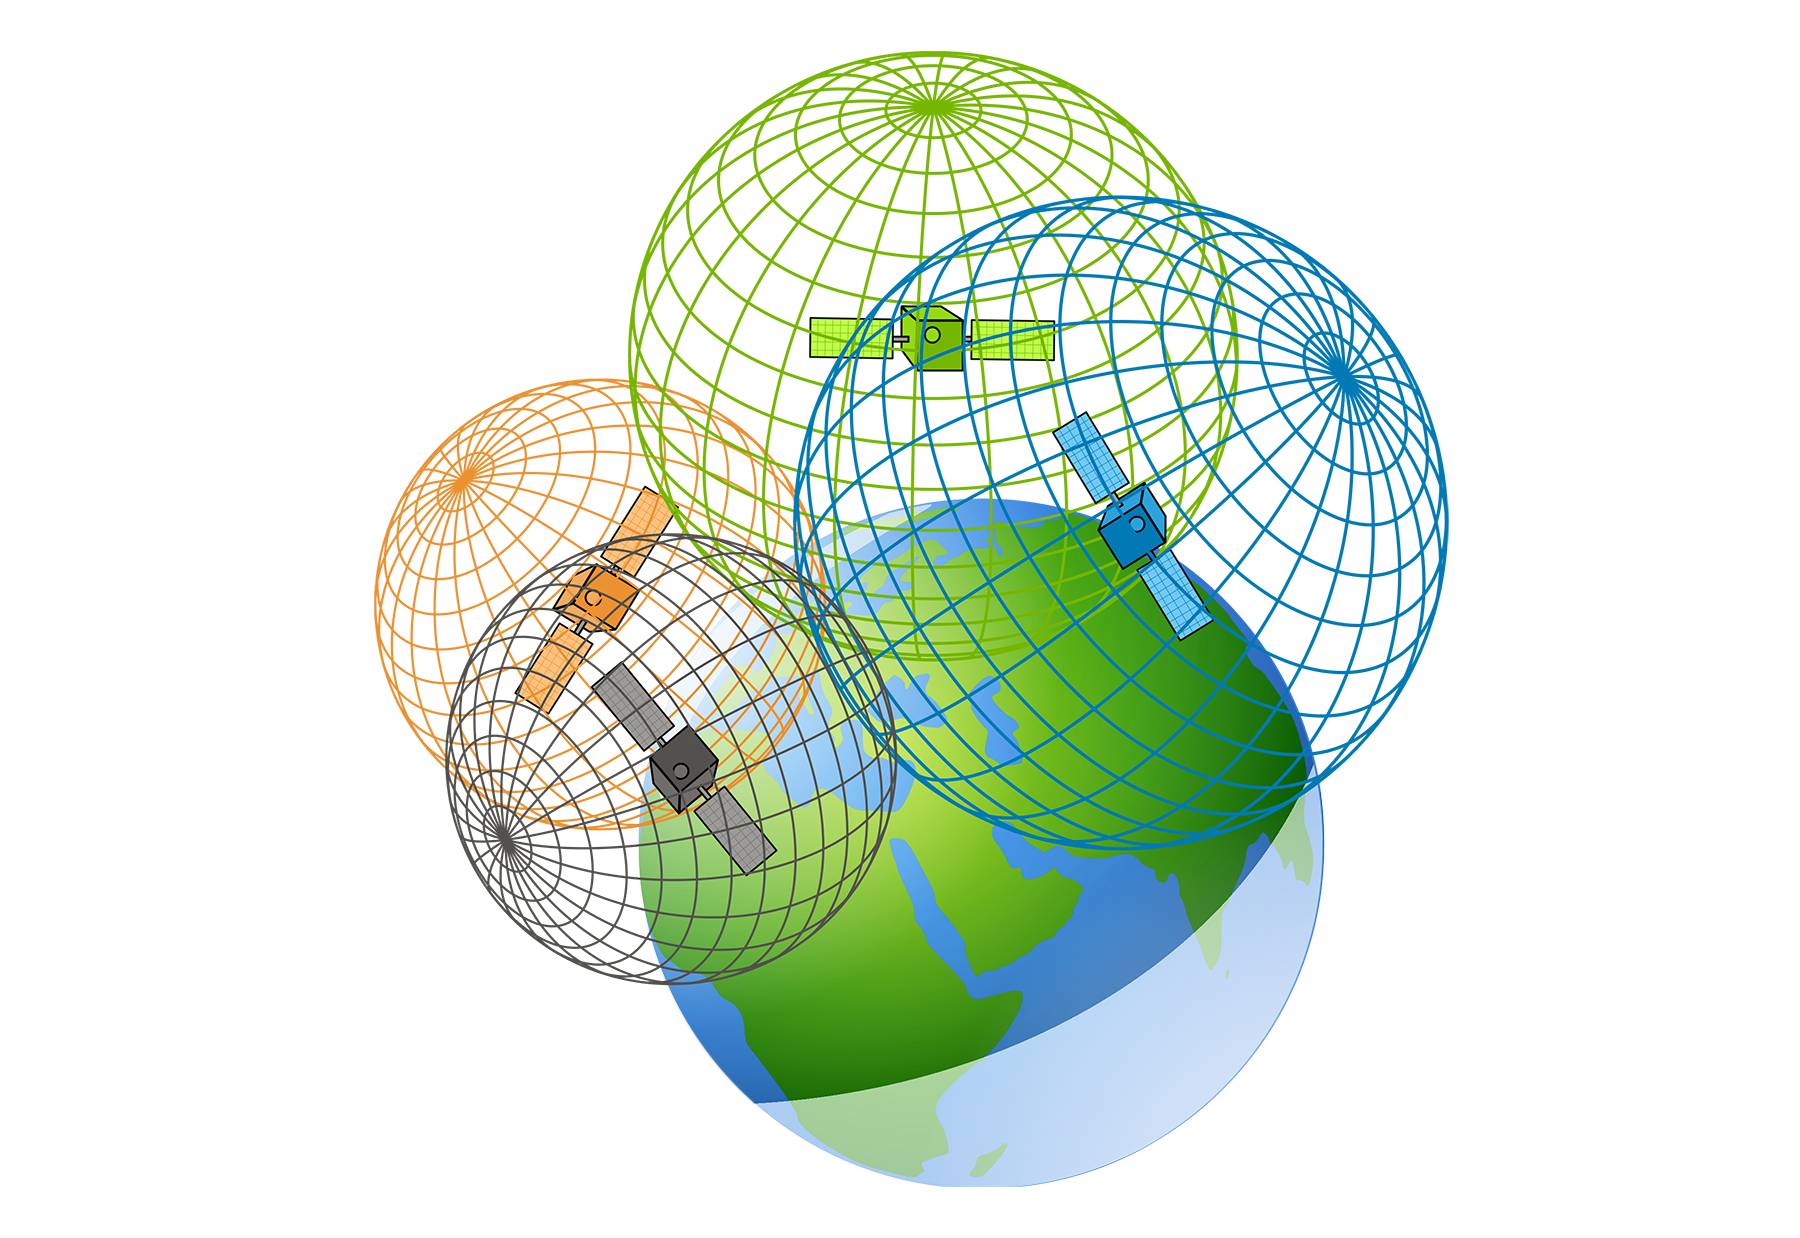
\includegraphics[width=0.9\textwidth]{img/GPS-Trilateration.png}
                \caption{GPS trilateration}
            \end{figure}

        \end{column}

        \begin{column}{0.5\textwidth}

            Basic math involved in trilateration:

            \begin{equation*}
                \Delta d_i = c \cdot \Delta t = c \cdot (t_{\text{sat}} - t_{\text{rcvr}})
            \end{equation*}

            Our system of equations has 4 unknowns:

            \begin{equation*}
                \underbrace{d_1, d_2, d_3, \Delta t}_\text{4 Unknowns requires 4 satellites}
            \end{equation*}

            \textbf{Final position strongly depends on $\Delta t$.}

        \end{column}

    \end{columns}

    \vspace{10pt}

    Because of better holdover capabilities, the use of a CSAC in the receiver allows to eliminate the need for the 4th satellite after the first clock calibration.

    A more accurate frequency of the receiver clock allows for a faster GNSS codes search and indeed a lower power consumption.

\end{frame}

\begin{frame}[allowframebreaks]{References}
    \nocite{*}
    \bibliography{references}
\end{frame}

\begin{frame}[standout]
    Questions?
\end{frame}

\begin{frame}[standout]
    Thank you!
\end{frame}

\end{document}